\documentclass[a4paper,12pt]{beamer}
\usepackage{tabularx}
\usepackage{array}
\usepackage{graphicx}
\usepackage{listings}
\usepackage{hyperref}
\usepackage{color}
\usepackage{tikz}

\usetikzlibrary{arrows.meta, positioning, shapes.geometric}

\usecolortheme{whale}

\definecolor{lightgray}{gray}{0.95}

\lstset{
    language=SQL,
    showspaces=false, 
    numbers=left,
    numberstyle=\tiny,
    backgroundcolor=\color{lightgray},
    keywordstyle=\color{blue}\bfseries,
    commentstyle=\color{gray},
    stringstyle=\color{orange},
    basicstyle=\ttfamily\scriptsize,
    breaklines=true,
    literate=
        {é}{{\'e}}1
        {è}{{\`e}}1
        {à}{{\`a}}1
        {ù}{{\`u}}1
        {ç}{{\c{c}}}1
        {ô}{{\^o}}1
        {ê}{{\^e}}1,
}

\title{TIPE : Optimisation de requêtes itérées d'une base de données orientée colonne}
\author[Eliott P \& Antoine BP]{Eliott Paquet \& Antoine Bertin--Paillette}
\date{2025}


% Barre Pied de page
\setbeamertemplate{footline}{
    \begin{beamercolorbox}[wd=\paperwidth,ht=2.25ex,dp=1ex]{author in head/foot}
    \usebeamerfont{author in head/foot}
    \hspace*{2ex}\insertshortauthor \hfill \inserttitle \hfill \insertdate \hfill \insertframenumber/\inserttotalframenumber\hspace*{2ex}
    \end{beamercolorbox}
}

% Barre d'en tête
\setbeamertemplate{headline}{%
    \begin{beamercolorbox}[ht=2.5ex,dp=1.125ex]{section in head/foot}%
        \insertsectionnavigationhorizontal{\paperwidth}{}{}%
    \end{beamercolorbox}%
    \begin{beamercolorbox}[ht=2.5ex,dp=1.125ex]{subsection in head/foot}%
        \insertsubsectionnavigationhorizontal{\paperwidth}{}{}%
    \end{beamercolorbox}%
}



\begin{document}
\begin{frame}
	\titlepage
\end{frame}

\section{Problématique}
\subsection{Les défauts des systèmes row-based}
\begin{frame}[containsverbatim]
	\frametitle{Les défauts des systèmes row-based sur les fonctions d'agrégation.}
	\begin{lstlisting}
Select SUM(purchase) /*fonction d'agrégation*/
From Sales;
\end{lstlisting}
	\begin{figure}[h]
		\centering
		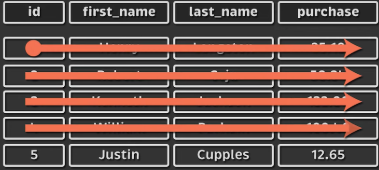
\includegraphics[width=200pt]{ressource/exemple_row_sucks.png}
		\caption{\small Il faut lire presque toutes les lignes pour traiter une fonction d'agrégation, ce qui augmente fortement le temps d'exécution.}
	\end{figure}

\end{frame}
\subsection{problématique}



\begin{frame}[containsverbatim] % Remove header/footer for full focus
	\frametitle{Problématique}
	\centering

	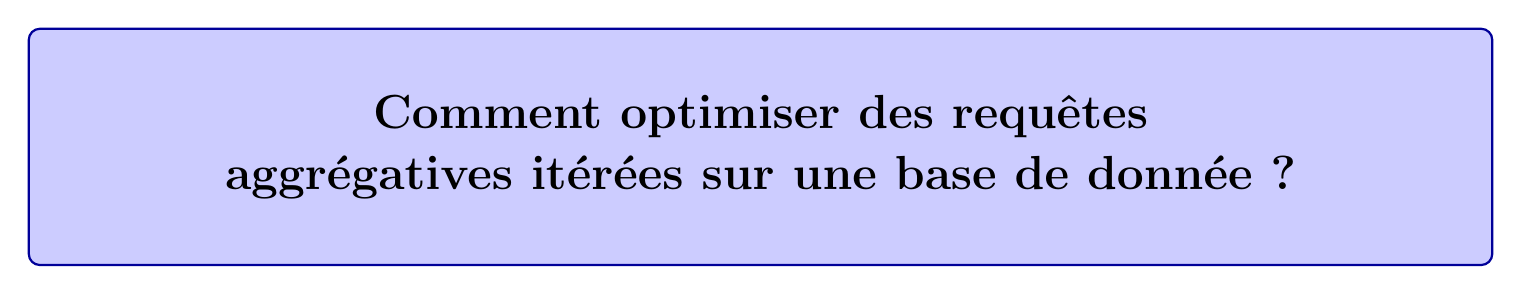
\begin{tikzpicture}
		\node[
			draw=blue!60!black,
			fill=blue!20,
			thick,
			rounded corners,
			text centered,
			text width=0.85\paperwidth,
			minimum width=0.85\paperwidth,
			minimum height=3cm,
			font=\LARGE\bfseries
		] (titlebox) {%
			Comment optimiser des requêtes aggrégatives
			itérées sur une base de donnée ?
		};
	\end{tikzpicture}



\end{frame}


\section{Notre approche}
\subsection{Les bases}
\begin{frame}
	\frametitle{Les bases de données orientées colonnes}
	\begin{figure}[h]
		\centering
		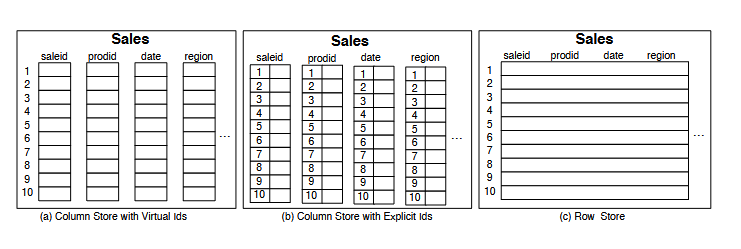
\includegraphics[width=300pt]{ressource/row_vs_column.png}
		\caption{Rendu physique des BDD orientées colonnes et BDD orientées lignes}
	\end{figure}
\end{frame}

\subsection{traitement d'une requête}
\begin{frame}
	\frametitle{Description du traitement d'une requête}
	\begin{figure}[h]
		\centering
		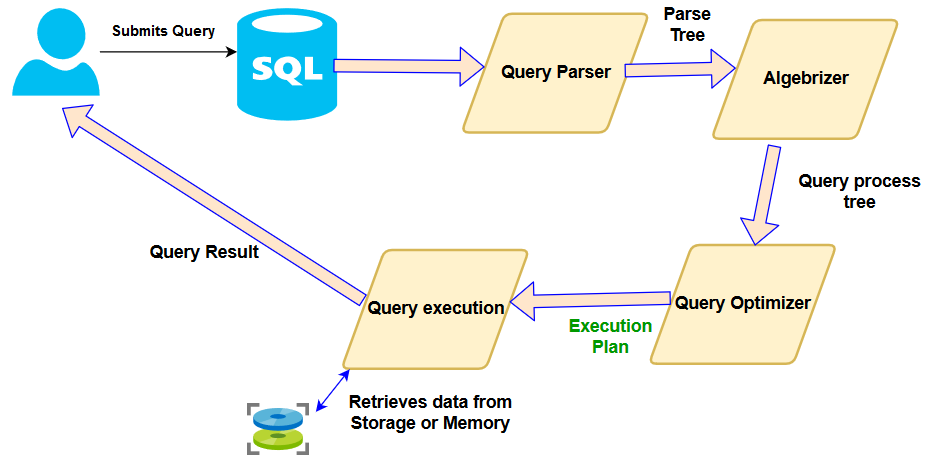
\includegraphics[width=300pt]{ressource/query_map.png}
		\caption{Voici (dans les grandes lignes) à quoi ressemble l'exécution d'une requête par une base de données.}
	\end{figure}
\end{frame}
\subsection{Idées d'optimisation }
\begin{frame}
	\frametitle{Procédés d'optimisation}


	\setlength{\tabcolsep}{8pt} % Marges internes dans les cases
	\renewcommand{\arraystretch}{2} % Hauteur des lignes (plus d’espace vertical)

	\begin{center}
		\begin{tabular}{|p{0.4\linewidth}|p{0.4\linewidth}|}
			\hline
			\textbf{La Vectorisation}                                              & \textbf{Décompression tardive}                    \\
			Consiste à traiter un vecteur de donnée pour les étapes de Sélection   &
			Pour certaine étape "facile" il est possible de traiter les données compressées                                            \\
			\hline
			\textbf{Matérialisation tardive}                                       & \textbf{Recherche de plan par estimation du coût} \\
			Regrouper les couples le plus tard possible pour accélérer l'exécution &
			Chercher un plan optimisé en estimant le temps d'exécution                                                                 \\
			\hline
		\end{tabular}
	\end{center}

\end{frame}



\subsection{Procédé Expérimental}
\begin{frame}
	\frametitle{Procédé Expérimental}

	\begin{center}
		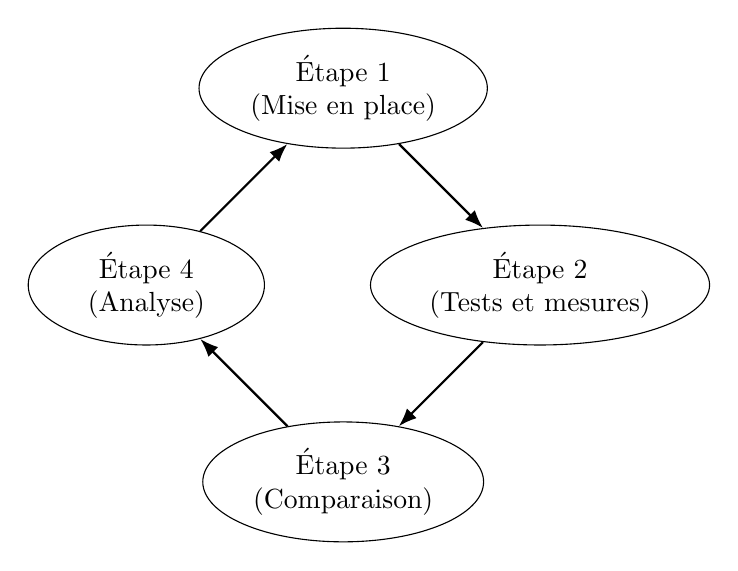
\begin{tikzpicture}[
				node distance=1.5cm,
				every node/.style={draw, ellipse, minimum width=3cm, minimum height=1.2cm, align=center},
				arrow/.style={-Latex, thick}
			]

			% Nodes arranged in a circle
			\node (a) at (90:2.5cm) {Étape 1\\(Mise en place)};
			\node (b) at (0:2.5cm)  {Étape 2\\(Tests et mesures)};
			\node (c) at (270:2.5cm) {Étape 3\\(Comparaison)};
			\node (d) at (180:2.5cm) {Étape 4\\(Analyse)};

			% Arrows
			\draw[arrow] (a) -- (b);
			\draw[arrow] (b) -- (c);
			\draw[arrow] (c) -- (d);
			\draw[arrow] (d) -- (a); % boucle

		\end{tikzpicture}
	\end{center}
\end{frame}


\subsection{Notre implémentation}
\begin{frame}
	\frametitle{L'avancement de notre implémentation}
	\begin{block}{Ce que nous avons réussi à implémenter}
		\begin{itemize}
			\item  Parseur/Lexeur de SQL
			\item  Stockage et lecture dans la mémoire
			\item  L'Exécution de la requête
		\end{itemize}
	\end{block}
	\begin{block}{Ce qu'il nous reste à faire}
		\begin{itemize}
			\item  L'Algebrizer
			\item  L'Optimisateur de requêtes
		\end{itemize}
	\end{block}
\end{frame}


\section{Conclusion}
\subsection{Notre objectif}

\begin{frame}
	\begin{figure}[h]
		\centering
		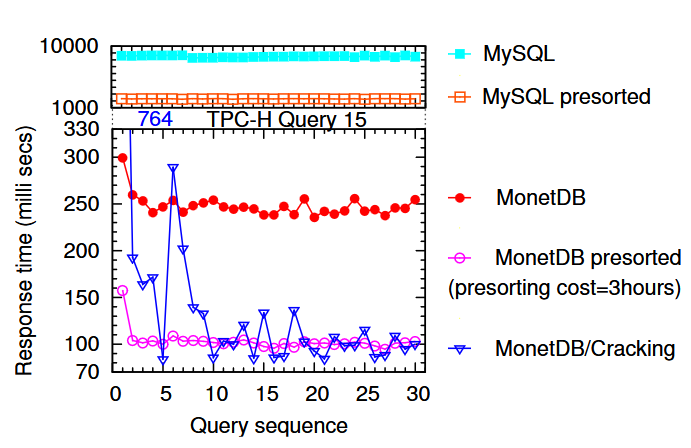
\includegraphics[width=300pt]{ressource/perf_comparaison.png}
		\caption{Notre objectif est de comparer avec ce genre de graphique notre implémentation et ce qui a déjà été fait.}
	\end{figure}
\end{frame}

\subsection{Nos ressources et contacts}
\begin{frame}
	\frametitle{Nos ressources et contacts}

	\textbf{Nos ressources :}
	\begin{itemize}
		\item \href{https://drive.google.com/file/d/1KNmuRBf8CV-s-zqdkUEP8iyYlPgFiglb/view?usp=drive_link}{\textit{The Design and Implementation of Modern Column-Oriented Database Systems}}
		\item \href{https://www.sqlite.org/docs.html}{La documentation de SQLite}
		\item \href{https://www.youtube.com/watch?v=LWS8LEQAUVc&list=PLSE8ODhjZXjYzlLMbX3cR0sxWnRM7CLFn}{Les cours du Prof. Andy Pavlo sur les SGBD et leur implémentation au CMU}
	\end{itemize}

	\medskip

	\textbf{Nos contacts :}
	\begin{itemize}
		\item \href{https://www.normalesup.org/~rouvroy}{Clément Rouvoy, étudiant ayant fait plusieurs stages sur les BDD en labo de recherche}
	\end{itemize}
\end{frame}
\end{document}